\chapter{Finite Markovian Lifts and Scalar Compression}\label{ch:lift}
A non-Markovian memory model and its finite Markovian approximation must be distinguished. A sum of exponential kernels introduces recursive OU factors. The full factor vector is Markovian; its weighted aggregate generally is not a closed scalar Markov process when decay rates differ. This chapter connects the kernel construction to the information discarded by a small control grid.
\section{Markovian Lifting}


\paragraph{Why lifting is needed.}

A Markov process has the property that the future depends on the present state alone. This is precisely what makes Brownian-motion-based models so efficient computationally: when one wants to generate the next step of the path, the whole history is not needed. By contrast, rough and fractional models are designed to preserve memory. In a Volterra representation,
\[
X_t=\int_0^t K(t,s)\,dW_s,
\]
the kernel \(K\) makes the current state depend on the entire past trajectory of the driving noise. This is mathematically attractive, but it destroys the simple recursive structure that is available in a Markov model.

One could always make the path itself part of the state, but that would not really solve anything. Expanding the state space to include the entire history is exact, yet it is not a simplification. The idea of Markovian lifting is more selective: instead of keeping the full path, one approximates the effect of the path by a finite collection of auxiliary state variables that are themselves Markovian. In this way, one retains the main covariance features of the rough dynamics without carrying the full historical trajectory at every step.

\subsection{Why exponentials are special}

The key mathematical reason lifting works is that exponentials satisfy a semigroup property. For any \(x>0\),
\[
e^{-x(t+\Delta t-s)} = e^{-x\Delta t}e^{-x(t-s)}.
\]
This simple identity is enough to recover a Markov recursion. To see it, define for a fixed rate \(x>0\) the auxiliary process
\[
U_t(x)=\int_0^t e^{-x(t-s)}\,dW_s.
\]
Then
\[
U_{t+\Delta t}(x)
=
\int_0^{t+\Delta t} e^{-x(t+\Delta t-s)}\,dW_s.
\]
Splitting the integral at time \(t\) and applying the semigroup property gives
\[
U_{t+\Delta t}(x)
=
e^{-x\Delta t}\int_0^t e^{-x(t-s)}\,dW_s
+
\int_t^{t+\Delta t} e^{-x(t+\Delta t-s)}\,dW_s,
\]
hence
\[
U_{t+\Delta t}(x)
=
e^{-x\Delta t}U_t(x)
+
\int_t^{t+\Delta t} e^{-x(t+\Delta t-s)}\,dW_s.
\]
The first term depends only on the current state \(U_t(x)\), while the second term depends only on the new Brownian increment over \([t,t+\Delta t]\). This is exactly the structure of a Markov update.

This mechanism fails for a pure power law. If one considers a rough kernel of the form
\[
(t-s)^{\alpha-1},
\]
then in general
\[
(t+\Delta t-s)^{\alpha-1}
\neq
(\Delta t)^{\alpha-1}(t-s)^{\alpha-1}.
\]
The semigroup property is absent, and this is the algebraic reason why pure rough kernels remain non-Markovian.

\subsection{Laplace representation of the rough kernel}

The rough-volatility kernel is typically written in the power-law form
\[
K_\alpha(\tau)=\frac{\tau^{\alpha-1}}{\Gamma(\alpha)},
\qquad
\alpha\in\left(\frac12,1\right),
\qquad
\tau>0.
\]
If one writes \(\alpha=H+\tfrac12\), then the rough regime corresponds to \(H\in(0,\tfrac12)\). The key observation behind lifting is that this kernel can be represented as a Laplace transform of exponential functions.

\begin{proposition}[Laplace representation of the power-law kernel]
For \(\alpha\in(0,1)\) and \(\tau>0\),
\[
\frac{\tau^{\alpha-1}}{\Gamma(\alpha)}
=
\frac{1}{\Gamma(\alpha)\Gamma(1-\alpha)}
\int_0^\infty e^{-\lambda \tau}\lambda^{-\alpha}\,d\lambda.
\]
Using Euler's reflection formula,
\[
\frac{1}{\Gamma(\alpha)\Gamma(1-\alpha)}
=
\frac{\sin(\pi\alpha)}{\pi},
\]
so equivalently
\[
\frac{\tau^{\alpha-1}}{\Gamma(\alpha)}
=
\frac{\sin(\pi\alpha)}{\pi}
\int_0^\infty e^{-\lambda \tau}\lambda^{-\alpha}\,d\lambda.
\]
\end{proposition}

\begin{proof}
By definition of the Gamma function,
\[
\Gamma(1-\alpha)=\int_0^\infty u^{-\alpha}e^{-u}\,du.
\]
Now make the substitution \(u=\lambda \tau\), so that \(du=\tau\,d\lambda\). Then
\[
\Gamma(1-\alpha)
=
\int_0^\infty (\lambda\tau)^{-\alpha}e^{-\lambda\tau}\tau\,d\lambda
=
\tau^{1-\alpha}\int_0^\infty \lambda^{-\alpha}e^{-\lambda\tau}\,d\lambda.
\]
Dividing both sides by \(\tau^{1-\alpha}\Gamma(\alpha)\Gamma(1-\alpha)\) gives
\[
\frac{\tau^{\alpha-1}}{\Gamma(\alpha)}
=
\frac{1}{\Gamma(\alpha)\Gamma(1-\alpha)}
\int_0^\infty e^{-\lambda\tau}\lambda^{-\alpha}\,d\lambda.
\qedhere
\]
\end{proof}

This identity is the analytical foundation of Markovian lifting. A singular power-law kernel can be interpreted as a continuous mixture of exponential kernels, and each exponential kernel corresponds to one mean-reverting Markov factor.

\subsection{From a continuous mixture to a finite lifted state}

The continuous Laplace representation is still infinite-dimensional. To obtain a practical model, one replaces the integral over \(\lambda\) by a finite quadrature rule. Choose rates
\[
\lambda_1,\dots,\lambda_M>0
\]
and positive weights
\[
w_1,\dots,w_M>0.
\]
Then approximate the rough kernel by
\[
K_\alpha(\tau)\approx K_\alpha^{(M)}(\tau)
=
\sum_{k=1}^M w_k e^{-\lambda_k \tau}.
\]
The corresponding lifted process becomes
\[
Y_t^{(M)}
=
\int_0^t K_\alpha^{(M)}(t-s)\,dW_s
=
\sum_{k=1}^M w_k U_t^{(k)},
\]
where
\[
U_t^{(k)}
=
\int_0^t e^{-\lambda_k(t-s)}\,dW_s.
\]
Each factor \(U^{(k)}\) is an Ornstein--Uhlenbeck-type Gaussian state satisfying
\[
dU_t^{(k)}=-\lambda_k U_t^{(k)}\,dt + dW_t,
\qquad
U_0^{(k)}=0.
\]
The entire lifted state is therefore
\[
Z_t=\bigl(U_t^{(1)},\dots,U_t^{(M)}\bigr)^\top,
\]
which is finite-dimensional and Markovian.

This is the core idea of lifting: instead of carrying an infinite-dimensional Volterra memory, one works with a stack of \(M\) mean-reverting factors. The model is no longer exact at finite \(M\), but it regains the recursive structure that is lost in the rough Volterra formulation.

\paragraph{Why this matters for rough volatility.}

The relevance of lifting is especially clear in rough-volatility models. A prototypical rough variance process may be written schematically as
\[
V_t
=
V_0
+
\int_0^t K_\alpha(t-s)\,dZ_s,
\]
where \(Z\) collects the drift and volatility-of-volatility terms. The non-Markovian difficulty comes entirely from the kernel \(K_\alpha\). Once \(K_\alpha\) is replaced by its finite exponential approximation \(K_\alpha^{(M)}\), the same variance process can be written as a linear combination of \(M\) Markovian factors:
\[
V_t
\approx
V_0+\sum_{k=1}^M w_k U_t^{(k)}.
\]
This is the step that restores the affine-type structure and makes fast simulation feasible again. In other words, lifting does not eliminate roughness by ignoring it; it replaces roughness by a structured finite-dimensional approximation that can still be handled recursively.

\subsection{Discrete-time recursion}

Fix a uniform grid
\[
t_i=i\Delta t,
\qquad i=0,\dots,n,
\qquad \Delta t=\frac{T}{n}.
\]
For each OU factor, the exact one-step transition is
\[
U_{i+1}^{(k)}=e^{-\lambda_k\Delta t}U_i^{(k)}+\eta_{i+1}^{(k)},
\]
where the innovation vector
\[
\eta_{i+1}=
\bigl(\eta_{i+1}^{(1)},\dots,\eta_{i+1}^{(M)}\bigr)^\top
\]
is centered Gaussian. Because all factors are driven by the same Brownian motion, these innovations are correlated, with covariance
\[
\Cov\!\bigl(\eta^{(j)},\eta^{(k)}\bigr)
=
\frac{1-e^{-(\lambda_j+\lambda_k)\Delta t}}{\lambda_j+\lambda_k}.
\]
After updating the factors, the lifted process is reconstructed by
\[
Y_i^{(M)}=\sum_{k=1}^M w_k U_i^{(k)}.
\]

An equivalent weighted-state representation is also possible. One may define
\[
X_t^{(k)}:=w_k U_t^{(k)},
\]
so that
\[
dX_t^{(k)}=-\lambda_k X_t^{(k)}\,dt+w_k\,dW_t,
\qquad
Y_t^{(M)}=\sum_{k=1}^M X_t^{(k)}.
\]
In that convention, the innovation covariance becomes
\[
\Cov\!\bigl(\eta^{(j)},\eta^{(k)}\bigr)
=
w_jw_k\,
\frac{1-e^{-(\lambda_j+\lambda_k)\Delta t}}{\lambda_j+\lambda_k}.
\]
Both formulations are equivalent as long as the weights are used consistently.

\subsection{Practical construction of the lift}

\paragraph{Rates and weights.}

The finite approximation depends on the choice of quadrature nodes \(\lambda_k\) and weights \(w_k\). A common practical heuristic is to use log-spaced rates,
\[
\lambda_k \in \left[\frac{2}{T},\frac{400}{T}\right],
\]
and weights proportional to
\[
w_k \propto \lambda_k^{-(H+\frac12)}.
\]
This mirrors the Laplace-domain mass of the rough kernel and usually provides a reasonable first approximation. However, this choice is heuristic rather than optimal. In particular, the approximation error is not guaranteed to decrease monotonically with \(M\), and in finite samples the empirical covariance RMSE may oscillate because of three interacting effects:
\begin{itemize}
    \item approximation error from the finite exponential mixture,
    \item Monte Carlo noise from the simulated covariance matrix,
    \item numerical conditioning effects when the factor system becomes larger.
\end{itemize}

For this reason, one should interpret the lifting dimension \(M\) as a bias--variance trade-off rather than as a parameter for which ``larger is always better''. In practice, a moderate value often gives the most stable overall result.

\paragraph{Discrete-time recipe.}

A convenient summary of the lifting procedure is the following:

\begin{enumerate}[label=\arabic*.]
    \item Choose a Hurst parameter \(H\in(0,1)\) and a lifting dimension \(M\).
    \item Define a time grid \(t_i=i\Delta t\) on \([0,T]\).
    \item Select mean-reversion rates \(\lambda_1,\dots,\lambda_M\), typically on a log scale.
    \item Choose weights \(w_1,\dots,w_M\) from a Laplace-domain quadrature heuristic.
    \item Build the Gaussian innovation covariance matrix of the OU factors.
    \item Simulate the factor recursion
    \[
    U_{i+1}^{(k)}=e^{-\lambda_k\Delta t}U_i^{(k)}+\eta_{i+1}^{(k)}.
    \]
    \item Aggregate the factors through
    \[
    Y_i^{(M)}=\sum_{k=1}^M w_k U_i^{(k)}.
    \]
\end{enumerate}

When the objective is to compare the lifted process directly with fractional Brownian motion on a fixed grid, it is often useful to rescale each time column so that the marginal variance matches
\[
\Var(B_t^H)=t^{2H}.
\]
This does not turn the lift into exact fractional Brownian motion. It simply isolates the covariance-shape approximation from a mismatch in marginal scale.

\paragraph{Implementation.}

This implementation keeps the OU factors unweighted internally and applies the weights only at aggregation. The function \texttt{match\_fbm\_marginals} can then be used when the goal is a direct visual or covariance comparison with fractional Brownian motion on a fixed discrete grid.

\subsection{Visual comparison across Hurst parameters}

The panels below illustrate the lifted approximation for three representative values of the Hurst parameter. In each composite image, the main lifted covariance is shown together with the target fractional covariance and a lag-wise covariance-error profile. The smaller diagnostic panels also compare nearby lifting dimensions, which makes it possible to see that the empirical error does not necessarily decrease monotonically as the number of OU factors changes.

The important point is therefore not a perfectly monotone RMSE sequence, but rather the overall stability of the approximation. Across repeated simulations, the empirical covariance error oscillates because it is itself a Monte Carlo object. 

The case $H=0.8$ is included as a persistent stress regime for the numerical comparison. It lies outside the standard empirically rough range $H<\tfrac12$ covered by the singular-kernel argument above, so it should not be read as a claim that persistent volatility is rough in the usual sense.

\begin{algorithm}[H]
\caption{Reading the Markovian-lifting diagnostic panels}
\DontPrintSemicolon
choose \(H\), a factor count \(M\), rates \(\lambda_k\), and weights \(w_k\)\;
simulate the correlated OU-factor recursion for the lifted state\;
aggregate \(Y^{(M)}=\sum_k w_k U^{(k)}\) and match the marginal scale when comparing with \(B^H\)\;
estimate the lifted covariance, compare it with the fractional target, and plot the lag-wise error\;
\end{algorithm}

Nevertheless, the error remains controlled, the qualitative geometry of the covariance surface is preserved, and the lift continues to reproduce the broad persistence pattern of the target process. In particular, the roughest regime is the hardest one to approximate, while smoother regimes are matched more easily.

\begin{figure}[H]
\centering
\begin{minipage}[t]{0.47\textwidth}
\vspace{0pt}
\normalsize

\vspace{0.25cm}

\textbf{Benchmark regime: \(H=0.5\).}

This is the intermediate benchmark case. The lifted covariance already captures the broad triangular structure of the target fractional covariance, but the lag-wise error profile shows that the approximation is still imperfect. The nearby factor-count diagnostics included in the panel also illustrate a practical point: changing the number of OU factors does not produce a strictly monotone reduction of the empirical RMSE. In repeated runs, the error oscillates because approximation error and Monte Carlo noise interact, but it remains controlled and the overall covariance geometry is preserved.

\end{minipage}
\hfill
\begin{minipage}[t]{0.47\textwidth}
\vspace{0pt}
\centering
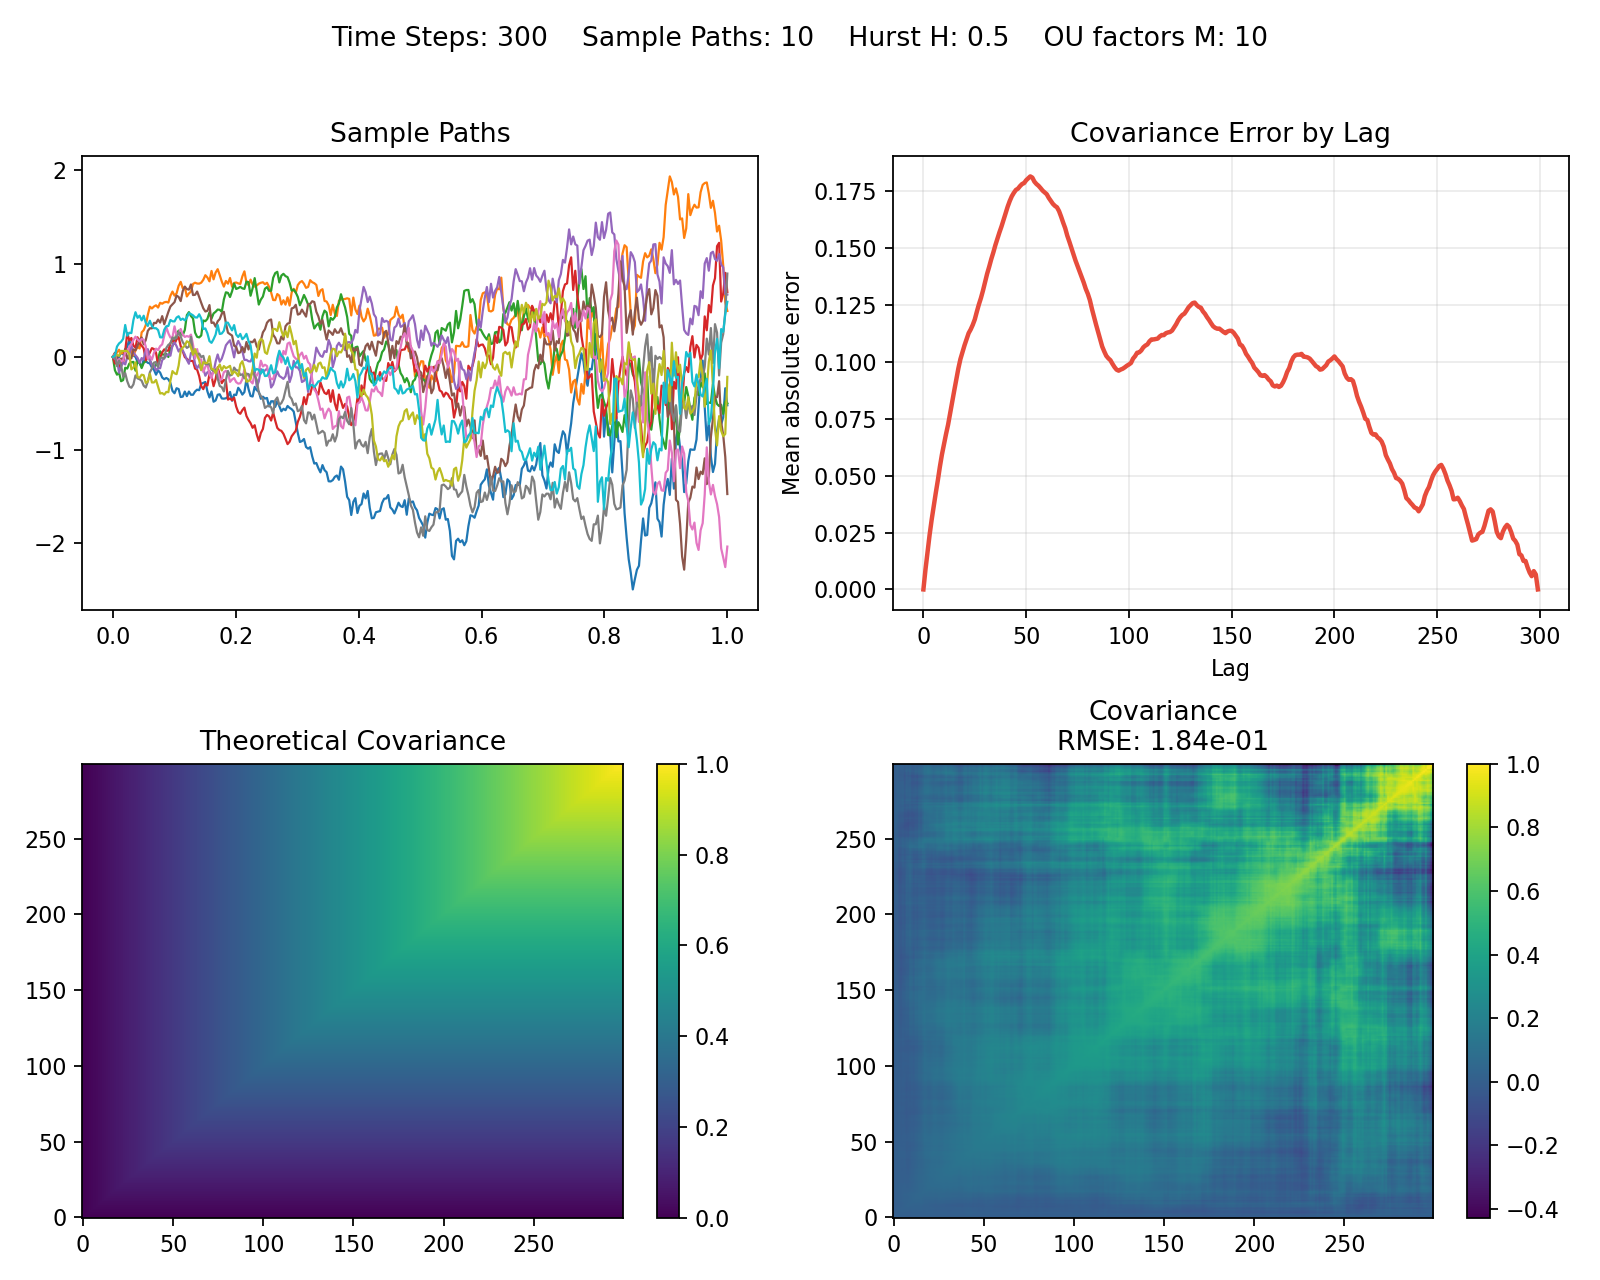
\includegraphics[width=6.5cm]{img/hft2-ML0_5.png}
\end{minipage}
\end{figure}

\begin{figure}[H]
\centering
\begin{minipage}[t]{0.47\textwidth}
\vspace{0pt}
\centering
%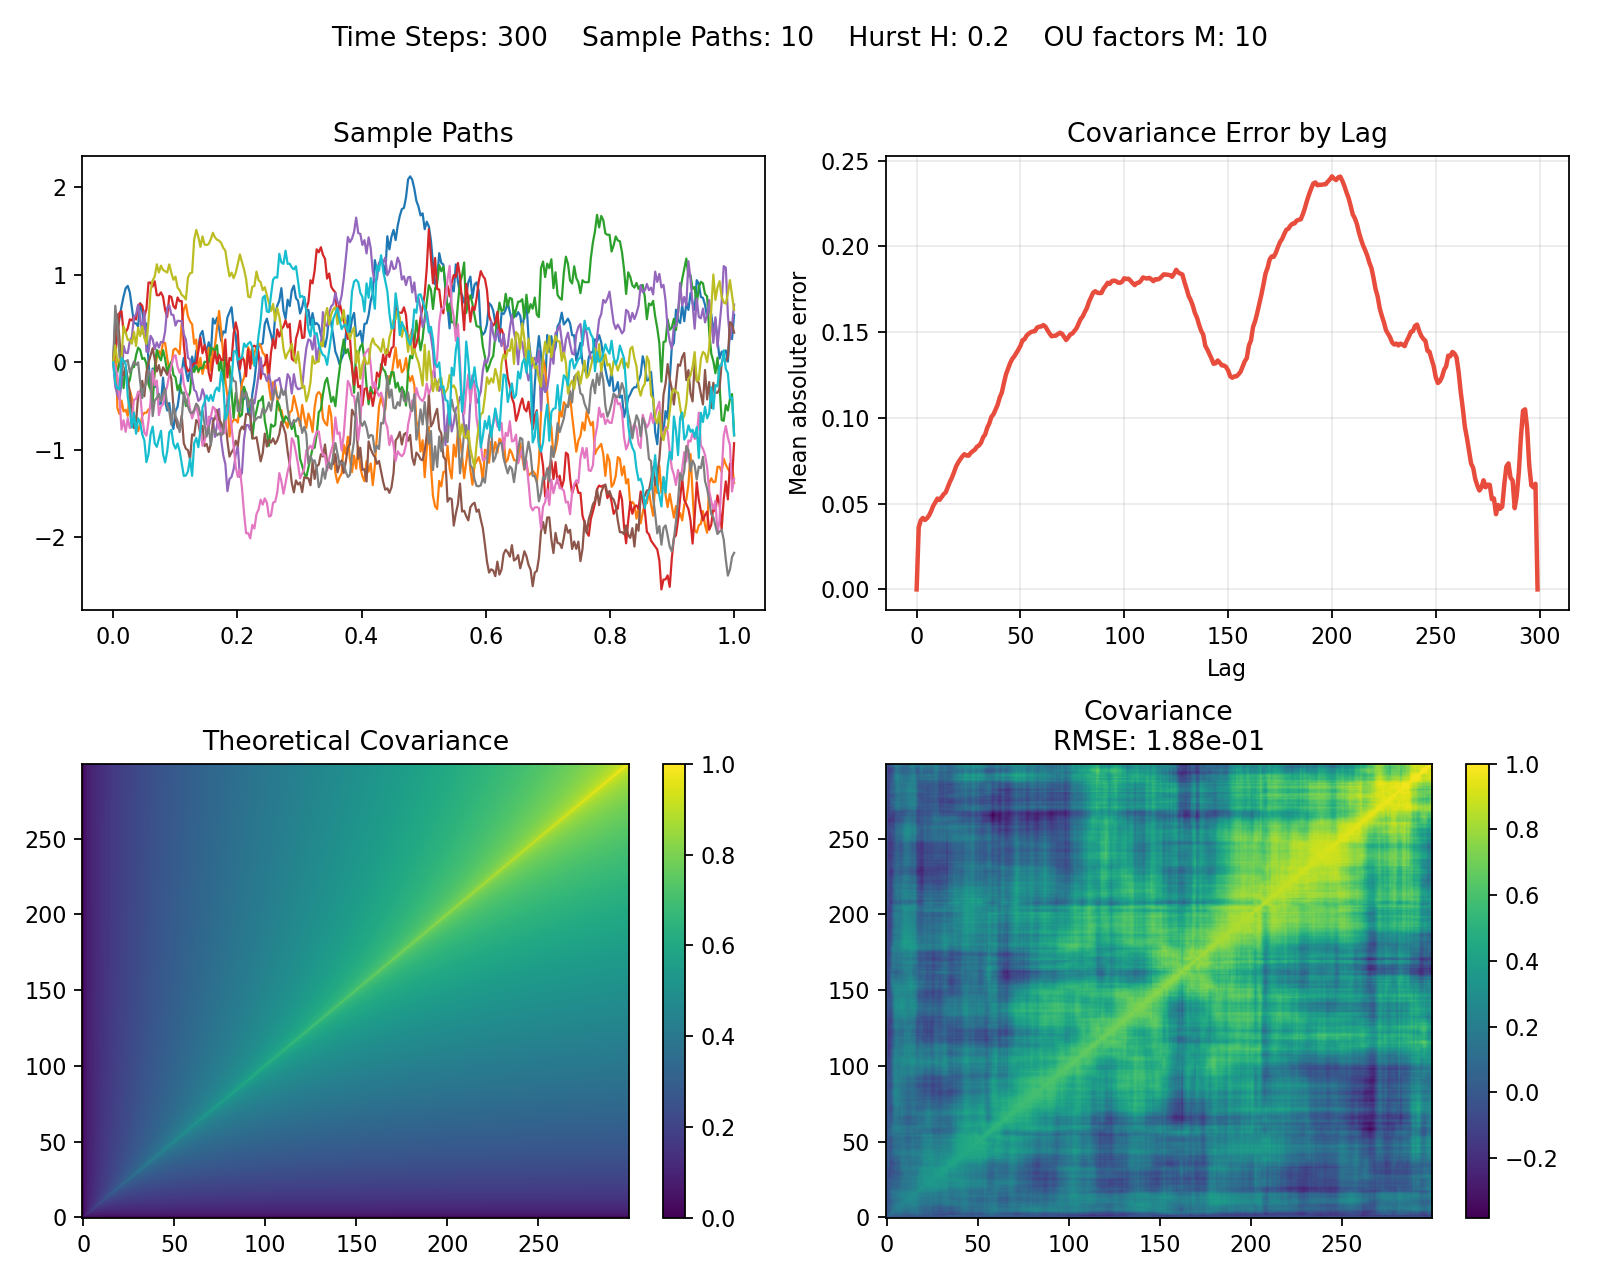
\includegraphics[width=\linewidth]{img/hft2-ML0_2.png}
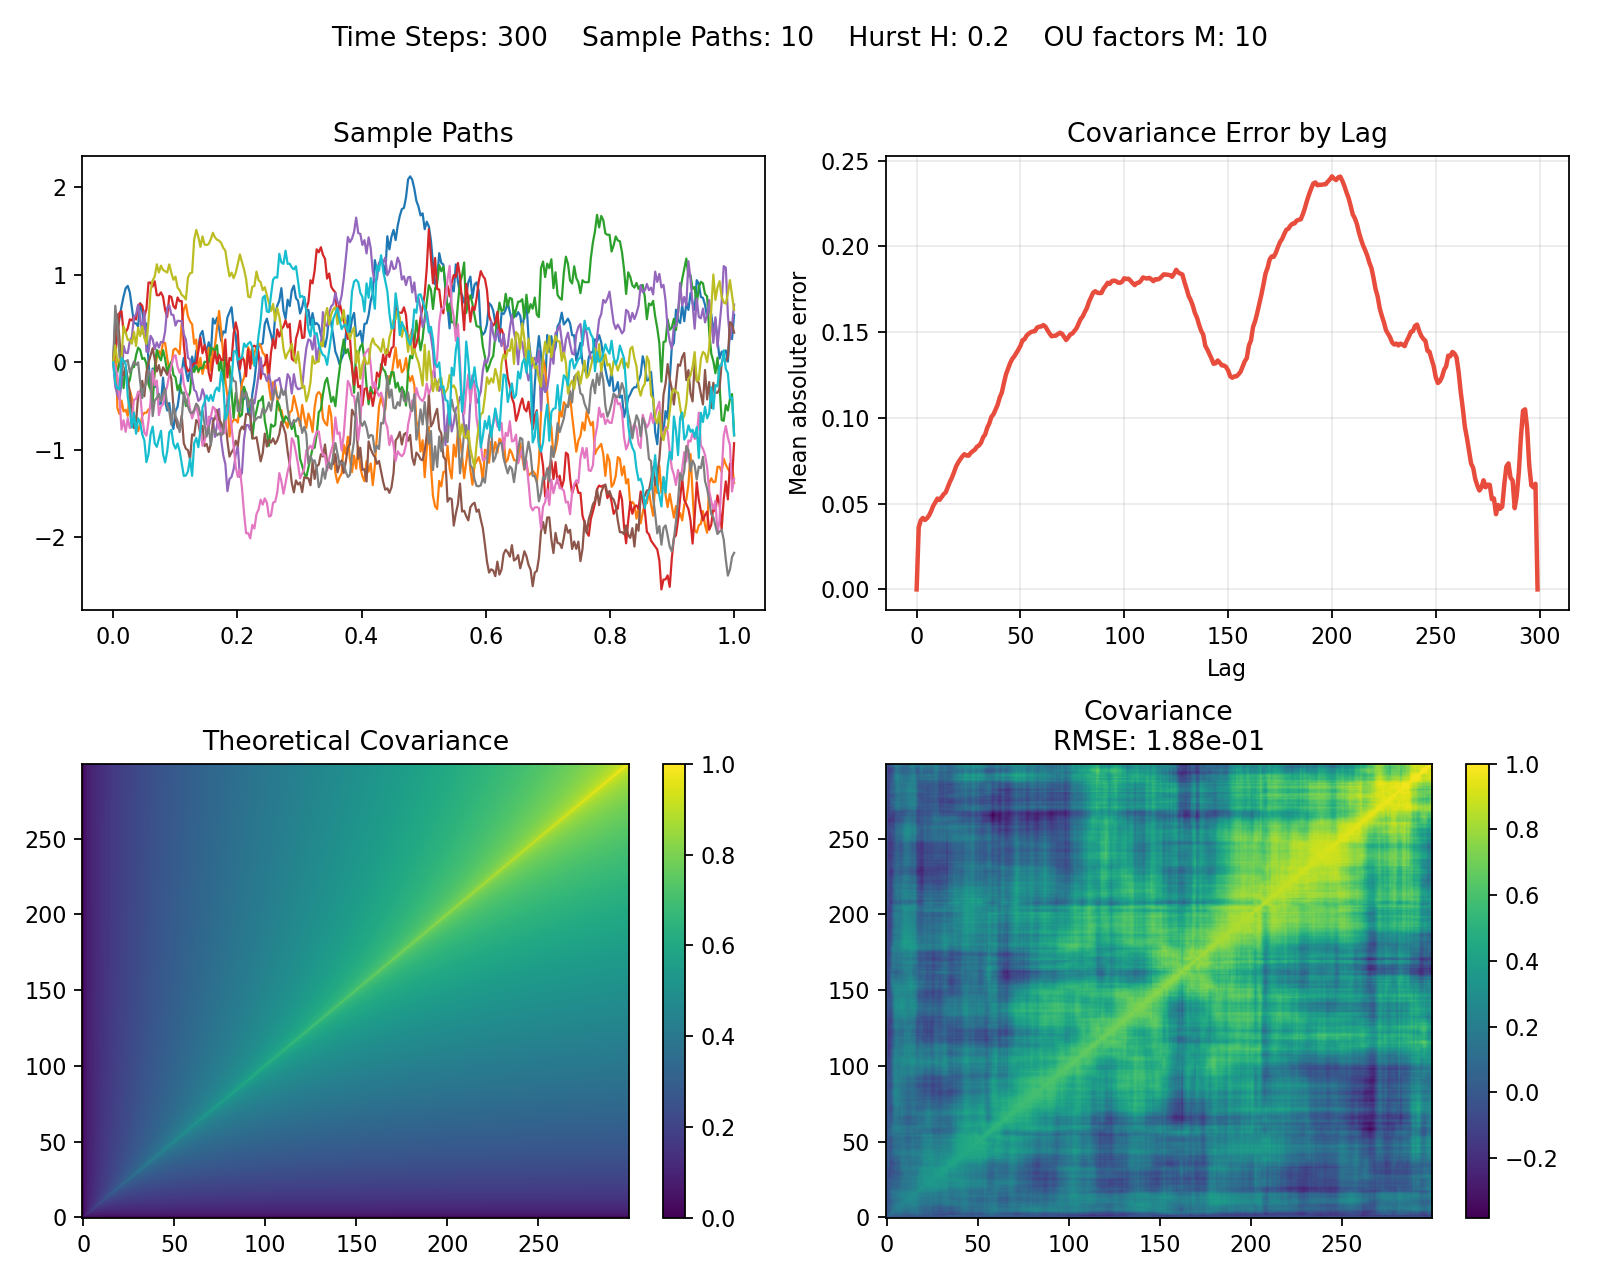
\includegraphics[width=6.5cm]{img/hft2-ML0_2.png}
\end{minipage}
\hfill
\begin{minipage}[t]{0.47\textwidth}
\vspace{0pt}
\normalsize
\textbf{Rough regime: \(H=0.2\).}

This is the most challenging case. Because the target covariance is generated by a much rougher kernel, a finite exponential mixture has a harder task: the lifted approximation still reproduces the global covariance pattern, but the empirical RMSE is larger and the lag-wise error is more pronounced. This should not be interpreted as a failure of the method. Rather, it shows that the roughest regime is the one in which the finite-dimensional approximation is under the greatest pressure. Even here, however, repeated simulation does not produce unstable behavior: %the error fluctuates from run to run, but remains bounded and the target covariance shape is still clearly recognizable.
\end{minipage}
\end{figure}

the error fluctuates from run to run, but remains bounded and the target covariance shape is still clearly recognizable.

\begin{figure}[H]
\centering
\begin{minipage}[t]{0.47\textwidth}
\vspace{0.25cm}
\normalsize
\textbf{Persistent regime: \(H=0.8\).}

When \(H>\tfrac12\), the target covariance is smoother and the lifted approximation becomes noticeably easier. This is reflected both in the heat maps and in the much smaller lag-wise covariance error. In this regime the exponential mixture is already rich enough to track the target geometry rather closely. As before, the RMSE observed in simulation is not perfectly deterministic across runs, but its oscillations remain small and the approximation is visibly more accurate than in the rough case.


\end{minipage}
\hfill
\begin{minipage}[t]{0.47\textwidth}
\vspace{0pt}
\centering
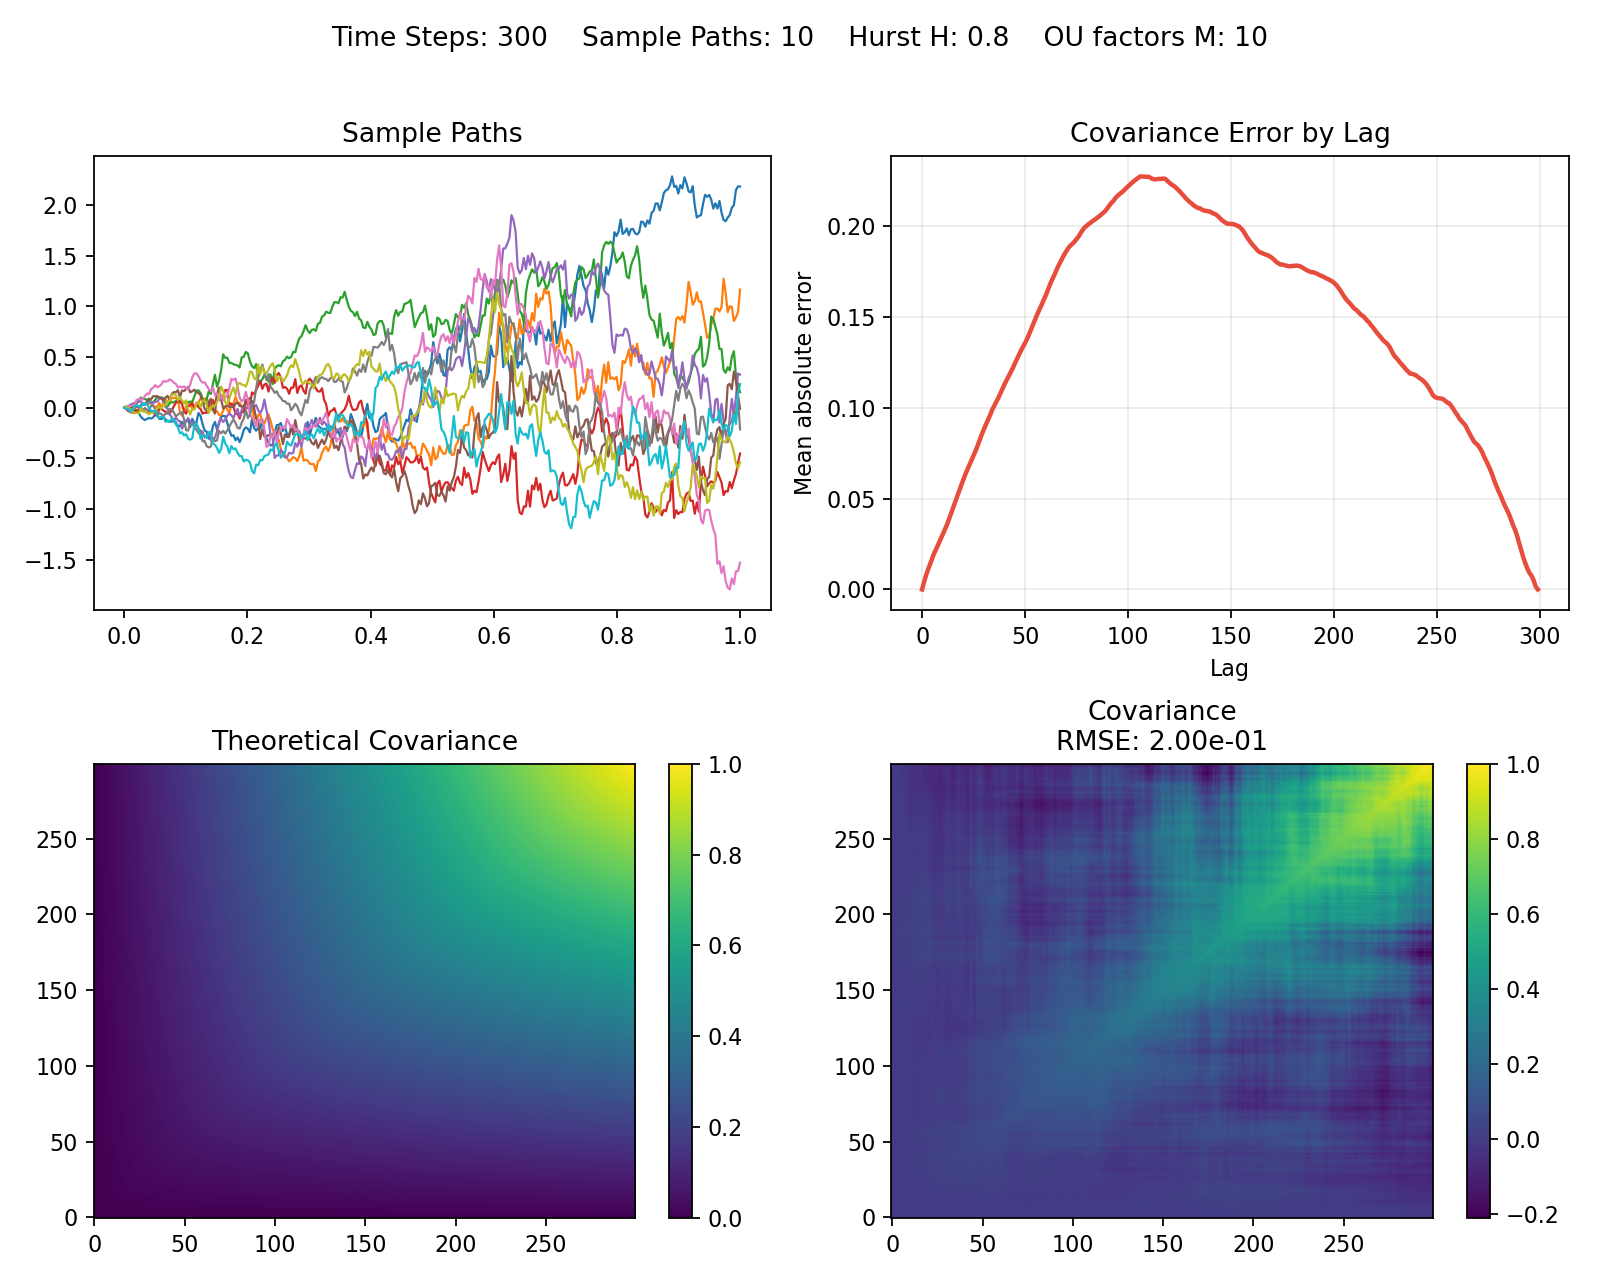
\includegraphics[width=6.5cm]{img/hft2-ML0_8.png}
\end{minipage}
\end{figure}

\subsection{What lifting solves, and what it does not solve}

Markovian lifting does not make the process exactly equal to fractional Brownian motion at finite \(M\). That would be too strong a claim. What it does is much more practical: it replaces a non-Markovian singular-memory dynamics by a finite-dimensional Markov approximation that preserves the main covariance features sufficiently well for simulation and control.

This distinction matters. The purpose of lifting is not exact identity at fixed factor dimension, but tractability. The rough memory is compressed into a finite state vector,
\[
Z_t=\bigl(U_t^{(1)},\dots,U_t^{(M)}\bigr)^\top,
\]
and this state can be updated recursively. That is precisely what makes the method attractive for repeated Monte Carlo simulation, calibration to liquid instruments, and eventually inventory control inside a market-making engine.

From the perspective of this study, Markovian lifting is therefore the final step in the mathematical transition
\[
\text{fractional covariance}
\quad\longrightarrow\quad
\text{causal Volterra representation}
\quad\longrightarrow\quad
\text{finite-dimensional Markov state}.
\]
The following volatility mapping uses this state-space perspective to reconnect the rough driver with a volatility process and, ultimately, with the reservation-price logic of a rough-volatility Avellaneda--Stoikov model.

\section{From Rough Paths to Rough Volatility}


The modeling task is now operational. A lifted rough state must be embedded inside a positive volatility process without breaking the recursive simulation architecture, and the resulting variance forecast must be translated into an inventory-aware quoting rule.

\subsection{From a lifted rough state to a volatility factor}

Let
\[
Y_t^{(M)}=\sum_{k=1}^M w_k U_t^{(k)}
\]
denote the lifted Gaussian rough state obtained in the previous chapter, where the factors \(U^{(k)}\) satisfy OU-type dynamics. By construction, \(Y_t^{(M)}\) is Gaussian and can take both positive and negative values. For that reason, it should not be interpreted directly as a variance process. A separate link function is needed to map the rough state into a positive volatility or variance input.

There are two natural modeling routes.

The first is structural and closer to the rough-Heston literature. In that case one thinks of volatility as a Volterra-type process driven by a rough kernel, for example
\[
V_t
=
V_0
+
\int_0^t
K_\alpha(t-s)
\Bigl(
\kappa(\theta-V_s)\,ds
+
\xi\sqrt{V_s}\,dW_s^v
\Bigr),
\qquad
K_\alpha(\tau)=\frac{\tau^{\alpha-1}}{\Gamma(\alpha)},
\]
with \(\alpha=H+\tfrac12\in(\tfrac12,1)\). This specification is conceptually important because it shows how rough memory enters variance directly. However, for the control problem it is not necessary to solve the full rough-Heston calibration problem in order to study market-making control.

The second route is more practical and better aligned with a simulation-first HFT study. One treats the lifted rough state as a latent Gaussian driver for log-volatility and defines, for example,
\[
\log v_t = m_t + \beta Y_t^{(M)},
\]
or equivalently
\[
v_t = \exp\!\bigl(m_t+\beta Y_t^{(M)}\bigr),
\]
where \(m_t\) is a deterministic baseline level and \(\beta>0\) controls the sensitivity of volatility to the rough factor. This choice guarantees positivity and preserves the intuition that large positive realizations of the rough state generate volatility clusters. It is also numerically convenient, because once the lifted factor has been simulated, the volatility process is obtained pointwise with no additional memory burden.

A slightly more stable centered version is
\[
v_t
=
\bar v\,
\exp\!\left(
\beta Y_t^{(M)}
-\frac12\beta^2\Var(Y_t^{(M)})
\right),
\]
which normalizes the unconditional level around \(\bar v\). The point is not that this is the only admissible specification, but that it turns the lifted state into a positive and simulation-ready volatility input.

\paragraph{Rough-volatility mid-price dynamics.}

Once a positive volatility process \(v_t\) has been constructed, the mid-price can be modeled by
\[
dS_t = \mu_t\,dt + \sqrt{v_t}\,dW_t^S,
\]
possibly with correlation between the price noise \(W^S\) and the volatility noise \(W^v\) or, in the lifted setting, between \(W^S\) and the Brownian driver behind the OU stack. At the level of the HFT engine, this is the natural rough-volatility replacement of the constant-\(\sigma\) benchmark studied in the Markovian diffusion benchmark.

The interpretation is immediate. In the classical model, the dealer faces a fixed local price-risk scale. In the rough version, this local risk scale fluctuates over time and does so with memory. Volatility can remain elevated for a while, calm periods can cluster together, and the price-risk forecast now depends on the current state of the rough factor rather than on a single constant parameter.

This is precisely where the rough-state machinery becomes relevant for quoting. The dealer does not need roughness for its own sake; the dealer needs a state variable that updates the perceived risk of carrying inventory. Once \(v_t\) is stochastic and persistent, the inventory penalty should react accordingly.

\subsection{A rough variance forecast for quoting}

The natural quantity entering an inventory-aware quoting rule is not just the instantaneous variance \(v_t\), but the remaining integrated variance over the control horizon. Define the conditional variance forecast
\[
\widehat{\Sigma}_{t,T}^2
:=
\mathbb{E}_t\!\left[\int_t^T v_u\,du\right].
\]
In the classical finite-horizon benchmark with constant volatility, this reduces to
\[
\widehat{\Sigma}_{t,T}^2 = \sigma^2(T-t).
\]
In the rough setting, however, the same object becomes state dependent:
\[
\widehat{\Sigma}_{t,T}^2
=
\widehat{\Sigma}_{t,T}^2\bigl(Z_t\bigr),
\qquad
Z_t=\bigl(U_t^{(1)},\dots,U_t^{(M)}\bigr)^\top.
\]
This is the key conceptual bridge from the lifted model to inventory control. The state vector \(Z_t\) summarizes the relevant memory of the volatility driver, and from this state one computes the forecasted risk scale that replaces the constant \(\sigma^2(T-t)\) of the original Avellaneda--Stoikov benchmark.

A practical rough-volatility reservation price can then be written as
\[
r_t^{\mathrm{rough}}
=
S_t-\gamma q_t\,\widehat{\Sigma}_{t,T}^2,
\]
with a corresponding spread proxy
\[
\psi_t^{\mathrm{rough}}
=
\frac{2}{k}
+
\gamma\,\widehat{\Sigma}_{t,T}^2.
\]
This keeps the notation consistent with the Markovian diffusion benchmark: \(S_t\) is the mid-price, \(q_t\) is inventory, \(\gamma\) is risk aversion, and \(k\) is the order-arrival sensitivity parameter. The only conceptual replacement is that the constant variance scale is upgraded to a state-dependent rough forecast. When \(v_t\equiv \sigma^2\), these formulas collapse back to the classical finite-horizon benchmark.

Hence the quoting rule becomes
\[
p_t^{ask}=r_t^{\mathrm{rough}}+\frac{\psi_t^{\mathrm{rough}}}{2},
\qquad
p_t^{bid}=r_t^{\mathrm{rough}}-\frac{\psi_t^{\mathrm{rough}}}{2}.
\]
This is not yet the exact optimal control for rough volatility, but it is the most natural extension of the classical inventory logic.

\subsection{Why the exact utility problem becomes difficult}

At this point one may ask whether the previous heuristic formulas can be justified directly from the same CARA-utility framework used in the classical Avellaneda--Stoikov model. Formally, the objective would still be
\[
\sup_{\pi}
\mathbb{E}\!\left[
-\exp\!\bigl(-\gamma(X_T+q_TS_T)\bigr)
\right],
\]
where \(\pi\) denotes the quoting policy. The problem is not the utility specification itself. Exponential utility remains a natural starting point because it preserves risk-aversion interpretability and fits well with marked-to-market wealth. The difficulty comes from the state dynamics.

Under rough volatility, the relevant Markov state is no longer just \((S_t,q_t)\), nor even \((S_t,q_t,v_t)\). Once lifting is introduced, the true state becomes
\[
(S_t,q_t,Z_t),
\qquad
Z_t\in\mathbb{R}^M.
\]
The value function is therefore of the form
\[
V(t,x,s,q,z)
=
\sup_{\pi}
\mathbb{E}_{t,x,s,q,z}
\!\left[
-\exp\!\bigl(-\gamma(X_T+q_TS_T)\bigr)
\right].
\]
Even though the lifted model is Markovian, it is Markovian in an enlarged state space of dimension \(M+3\) once cash is included. The corresponding HJB equation becomes substantially more complex than in the constant-volatility case.

Several specific difficulties arise.

First, the volatility process is now state dependent and persistent. This means that the continuation value depends not only on current inventory and current price, but also on the entire vector of lifted factors. The simple separation arguments used in the classical benchmark no longer go through cleanly.

Second, the arrival intensities and the price risk interact in a richer way. A dealer who sees a high-volatility rough state should generally quote more cautiously, but the best way to do so depends on how the execution intensities respond to the resulting spread changes. This turns the control problem into a coupled trade-off between inventory risk and fill risk in a higher-dimensional state space.

Third, if one allows correlation between the price Brownian motion and the volatility driver, the HJB acquires additional cross terms. Even when such correlation is ignored, the volatility forecast entering the value function is no longer deterministic.

Fourth, the exact optimal policy may not admit a closed-form expression. In the classical arithmetic Brownian benchmark, one obtains explicit or near-explicit reservation-price formulas because the value function retains a simple structure. Under rough volatility, even after lifting, there is no guarantee that the same exponential-affine ansatz will survive.

For these reasons, the utility problem remains well defined but analytically much less tractable. The lifting step restores Markovianity, not closed-form solvability.

\paragraph{Practical approximations to the control problem.}

The absence of a simple closed form does not make the model unusable. It only changes the level at which one works. Instead of insisting on a fully explicit optimal policy, one can proceed through structured approximations.

A first possibility is the \emph{frozen-state approximation}. One computes the conditional integrated variance forecast \(\widehat{\Sigma}_{t,T}^2\) from the current lifted state and plugs it into the classical reservation-price and spread formulas. This yields a quoting rule that is state dependent, causal, and easy to simulate.

A second possibility is simulation-based policy evaluation. One fixes a family of quoting rules parameterized by a small set of coefficients, simulates the marked-to-market utility under the rough-volatility engine, and then optimizes the coefficients numerically. In this approach, the lifted state is still essential because it allows recursive simulation without having to carry the full path.

A third possibility is to solve the HJB numerically on a reduced state grid, possibly after dimensionality reduction on the OU factors. This is more ambitious, but it is conceptually consistent with the lifted formulation.

The common theme is that the exact utility problem may lose analytical tractability, yet the lifted state keeps the model numerically accessible. This is precisely why the previous chapters were needed: without causality and without Markovian lifting, even these approximations would become cumbersome.

\subsection{Comparison with the naive benchmark from the Markovian diffusion benchmark}

The most natural practical comparison for the control problem is not against the exact rough-optimal policy, which may be unavailable in closed form, but against the same naive benchmark already used in the Markovian diffusion benchmark. This keeps the notation, accounting, and execution logic fixed while changing only the volatility module.

In the naive symmetric policy, the dealer ignores both inventory and rough volatility and posts
\[
p_t^{bid,\mathrm{naive}} = S_t-\bar\delta,
\qquad
p_t^{ask,\mathrm{naive}} = S_t+\bar\delta,
\]
with \(\bar\delta\) constant or deterministic. This is the same baseline used in the classical article. It provides a clean benchmark because it separates spread capture from active risk control.

The rough inventory-aware policy preserves the same state variables but replaces the constant risk scale with the rough variance forecast:
\[
p_t^{bid,\mathrm{rough}} = r_t^{\mathrm{rough}}-\frac{\psi_t^{\mathrm{rough}}}{2},
\qquad
p_t^{ask,\mathrm{rough}} = r_t^{\mathrm{rough}}+\frac{\psi_t^{\mathrm{rough}}}{2}.
\]
Hence the comparison with the Markovian diffusion benchmark is conceptually straightforward.

\begin{center}
\begin{tabularx}{\textwidth}{@{}lX@{}}
\toprule
Naive policy & Symmetric quotes around \(S_t\), no inventory correction, no rough-risk correction \\
Rough inventory-aware policy & Quotes centered around \(r_t^{\mathrm{rough}}\), with spread and skew driven by \(\widehat{\Sigma}_{t,T}^2(Z_t)\) \\
\bottomrule
\end{tabularx}
\end{center}

This comparison matters because rough volatility changes the environment in which the policy operates. In quiet periods, the naive policy may be overly conservative relative to the actual local risk. In clustered high-volatility periods, it may become too aggressive, keeping quotes too tight exactly when inventory is most dangerous. The rough-aware policy reacts to this state dependence by widening or skewing quotes according to the current volatility forecast.

The expected qualitative outcome is therefore the following. Relative to naive symmetric quoting, a rough-aware inventory rule should:
\begin{itemize}
    \item reduce inventory excursions when volatility clusters upward,
    \item stabilize marked-to-market wealth by reacting to persistent risk states,
    \item preserve more coherent quote behavior across regimes of calm and stress.
\end{itemize}
This is the rough-volatility analogue of the main lesson from the Markovian diffusion benchmark. In the classical benchmark, inventory-aware quoting dominated naive quoting because it reacted to inventory. In the present rough setting, the natural extension is that quoting should react both to inventory and to the current memory-driven risk scale.

\paragraph{Role of this chapter in the overall project.}

The causal construction and factor recursion above identify the volatility information supplied to the dealer. The variance forecast then connects this state to the reservation-price mechanism of the diffusion benchmark. This modeling bridge does not solve the full rough-volatility HJB: it identifies the state and the risk forecast whose full and reduced control generators must be distinguished next.

This is enough to define the architecture of the memory-dependent volatility model. The mid-price dynamics are upgraded from a constant-volatility diffusion to a rough-volatility diffusion; the reservation price is upgraded from a constant-variance inventory correction to a rough forecast correction; and the baseline comparison remains the same as in the Markovian diffusion benchmark, namely naive symmetric quoting versus inventory-aware quoting. What changes is the risk engine behind the quotes.

In this sense, the present chapter is the operational hinge of the paper. The earlier chapters supplied the rough mathematical state. This chapter turns that state into a volatility module. The remainder of the paper can therefore focus on validation, implementation, and numerical comparison rather than on rebuilding the rough machinery from scratch.

\subsection{Implementation and validation workflow}

Three numerical layers are now available, and they should be treated as complementary rather than competing constructions.

\begin{center}
\begin{tabularx}{\textwidth}{@{}lX@{}}
\toprule
Method & Best use \\
\midrule
Direct covariance / Cholesky & Ground-truth benchmark for checking Gaussian covariance and marginal scaling \\
Causal Volterra discretization & Conceptual simulation of rough memory with explicit path dependence \\
Markovian lifting & Fast repeated simulation, state recursion, and control-oriented implementation \\
\bottomrule
\end{tabularx}
\end{center}

Before embedding the rough module inside a quoting engine, the following checks should be passed:
\begin{enumerate}[label=\arabic*.]
    \item \textbf{Marginal scaling:} verify numerically that \(\Var(X_t)\) follows the intended \(t^{2H}\)-type behavior.
    \item \textbf{Covariance structure:} compare empirical and theoretical covariance heatmaps on a fixed time grid.
    \item \textbf{Stability in \(n\):} refine the time grid and confirm that discretization error decreases.
    \item \textbf{Stability in paths:} increase the number of Monte Carlo paths and verify convergence of empirical moments.
    \item \textbf{State update consistency:} for the lifted model, confirm that the OU recursion reproduces the intended covariance shape as \(M\) increases.
\end{enumerate}

\paragraph{Research workflow for the HFT project.}

A coherent workflow for the project is then:
\begin{enumerate}[label=\arabic*.]
    \item validate the classical Avellaneda--Stoikov engine under standard diffusions;
    \item add a rough-volatility module and keep execution and accounting unchanged;
    \item impose end-of-day netting and a liquidation-aware terminal accounting rule;
    \item compare naive symmetric quoting with inventory-aware quoting under rough variance;
    \item stress test sensitivity to \(H\), horizon length, path count, liquidation parameters, and lift dimension \(M\).
\end{enumerate}

\begin{algorithm}[H]
\small
\caption{From rough driver to market-making simulation}
\DontPrintSemicolon
choose horizon \(T\), grid size \(n\), Hurst parameter \(H\), and lift dimension \(M\)\;
specify rates \(\lambda_k\), weights \(w_k\), inventory, cash, and mid-price initial values\;
\For{\(i=0,\dots,n-2\)}{
  update the lifted factors, aggregate \(Y_{i+1}=\sum_{k=1}^M w_k X_{i+1}^{(k)}\), and map it into variance\;
  update the mid-price, compute the inventory-aware quotes, sample executions, and update state variables\;
}
mark wealth to market, liquidate residual inventory when required, and record PnL diagnostics\;
\end{algorithm}

This connects the volatility-state construction to the full/reduced control equations. The rough driver has now been defined, made causal, compressed into a lifted state, and translated into a volatility forecast. The remaining questions concern both the full control generator and policy behavior under liquidation; the next two chapters declare the equations and numerical conventions before assessing performance.
\section{Lifted HJB and State-Compression Defects}


Let $Z\in\mathbb R^M$ be the lifted volatility state and $Y=w^\top Z$ its aggregate. After separating cash and price under the assumptions specified in the full lifted model below, write the certainty-equivalent adjustment as $\theta(t,q,Z)$. The reduced calculation replaces this object by $\theta_0(t,q,Y)$. Its embedding into the full state is
\[
 \widetilde\theta_0(t,q,Z)=\theta_0(t,q,w^\top Z).
\]
This is a composition of functions, not a statement that $Y$ is Markovian. In particular, the aggregate drift generally depends on the entire factor vector. Two states with the same $Y$ may therefore have different continuation dynamics.

\subsection{Two residuals and their difference}
For a specified full operator $\mathcal H_F$ and reduced operator $\mathcal H_R$, define
\[
 R_F=\mathcal H_F[\widetilde\theta_0],\qquad
 R_R=\mathcal H_R[\theta_0],\qquad D=R_F-R_R.
\]
The first quantity tests the embedded baseline against the full model. The second tests it against the equation it was intended to solve. The difference isolates the operator discrepancy only when all remaining terms, conventions and evaluation points agree. A large $R_F$ cannot be attributed to state compression if $R_R$ is already large.

For smooth scalar functions, the chain rule gives
\[
 \partial_{z_i}\widetilde\theta_0=w_i\theta_{0,y},\qquad
 \partial_{z_i z_j}\widetilde\theta_0=w_iw_j\theta_{0,yy}.
\]
These identities avoid a high-dimensional finite-difference grid for the initial diagnostic. They do not eliminate the need to validate the scalar derivatives, boundary treatment and time discretization. The first implementation interpolates previously computed scalar derivatives; it does not claim they are derivatives of a globally smooth interpolant.

The following section records the proposed correction architecture. Its role is to organize a research method; the financial operator itself is derived independently in the full lifted model section.

The scalar policy is thus a computational approximation inside a finite Markovian environment, not a solution of the original non-Markovian problem. The next chapter writes the full and reduced generators under matching controls so that this information loss can be measured rather than hidden in calibration.
